% !TeX root = ../main.tex
% Add the above to each chapter to make compiling the PDF easier in some editors.

\chapter{Introduction}\label{chapter:introduction}


With the clean energy transition currently taking place in Europe with ambitious targets for 2030 and beyond \cite{EU_RE_Targets_2023}, wind energy is playing a central role in that transition and expected to rise to 50 \% in the EU energy mix \cite{ConsiliumEU_Harnessing_Wind_Power_2024}. 
With wind energy thus expected to become one of the main contributors to the EU's energy production and large potentials identified for both onshore and offshore parks \cite{EEA_Wind_Energy_Potential_2009}, attempts to optimize all parameters of windparks that result in even minor power efficiency improvement can be expected to yield significant returns in absolute power due to the scale of future wind energy production. 

Within the main wind energy challenges lies the problem of optimizing the layout of wind farms. Here, the main goal is to reduce the negative impact that wake effects between wind turbines have on overall power generation, with yield reduction of up to $15\%$  mainly due to reduced wind speeds in wake regions. Optimizing the farm for overall minimal wake exposure between wind turbines can thus potentially significantly increase the power output \cite{hou_review_2019,KIM2024123383}.

The problem reduces to placing wind turbines within a predefined zone, subject to the wind conditions as shown in Figure \ref{fig:intro_plot}. These wind conditions can be assumed to be deterministic or (more accurately) random variables, by considering probability distributions for variables like wind direction and wind speed.


\begin{figure}[h] 
	\centering
	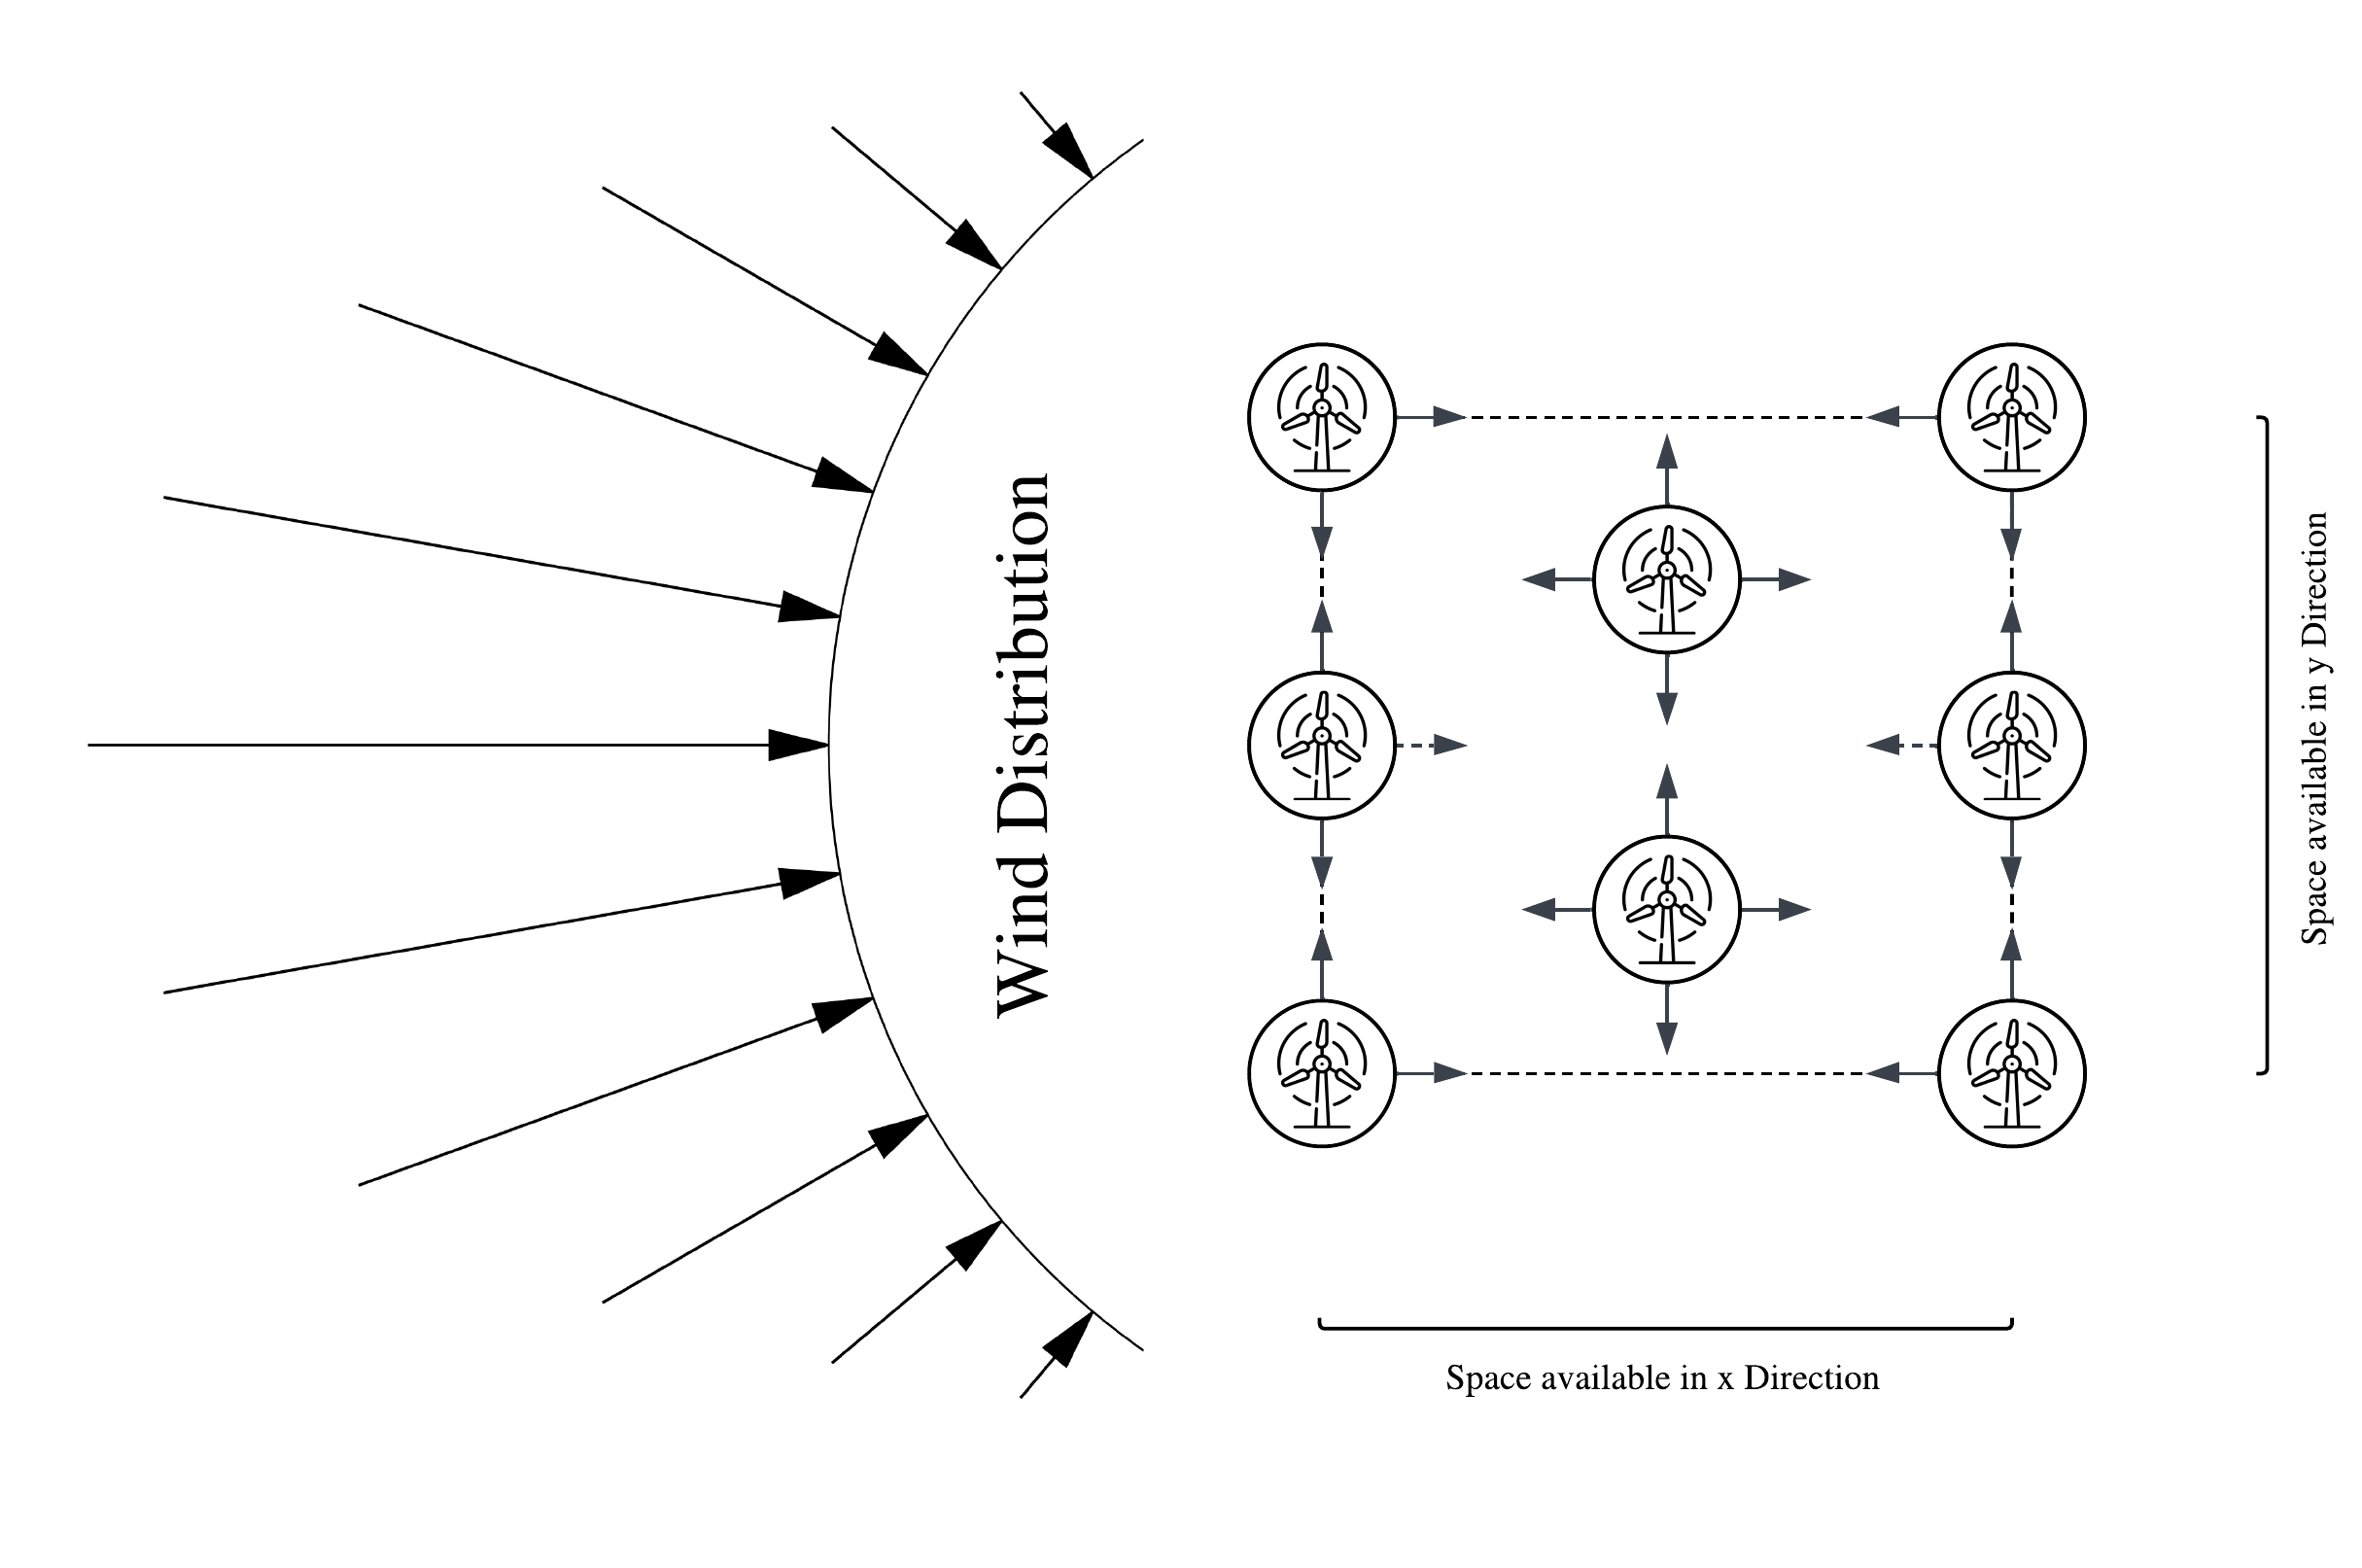
\includegraphics[width=1\textwidth]{../figures/introduction/intro_plot.png} 
	\caption{Optimizing the total power output of a farm reduces to placing wind turbines within a set space for the farm, subject to the wind conditions at the given location}
	\label{fig:intro_plot}
\end{figure}

In mathematical terms, this problem can be expressed as the attempt to maximize the sum of power output across all turbines, e.g., maximizing total farm output, subject to the limitations of the defined space, which is assumed to be rectangular: 

\begin{align}
	\max_{\mathbf{x}, \mathbf{y}} & f_{Power}(x_i, y_i, \text{wind conditions}) \\
	\text{s.t.} \quad 
	&  0 \leq x_i \leq X_{\max} \\
	&  0 \leq y_i \leq Y_{\max} \\
\end{align}

where:
\begin{itemize}
	\item \( (x_i,  y_i) \) are the positions of the turbines
	\item \( f_{Power, \text{NN}}(\cdot)\) is a neural network approximating the farm power output, e.g. the sum of power generated by all individual turbines
	\item \(  X_{\max}, Y_{\max} \) define the maximal extension of the space in which the turbines can be placed
	\item \(\textit{wind conditions}\) are the the random variables that represent the wind conditions at a specific location, like wind direction and wind speed with their respective probability distributions 
\end{itemize}


This thesis is dedicated to a new approach for optimizing the placement of a fixed number of wind turbines in a predefined space, beginning with the two-turbine problem, the problem of optimally placing two turbines relative to each other. To solve this optimization problem, an extension to the Pyomo Python library is used, which allows the embedding of Neural Networks into the optimization problem as a set of constraints \cite{ALCANTARA2023120895}. This extension allows the modelling of the effects of wind turbine placement relative to each other on power production. Introducing this model into the problem then allows for the optimization of overall power production across all wind turbines in the wind park.

To create a model that optimally fits to the needs of the optimization problem, the model is trained on data specifically generated with the \href{https://www.nrel.gov/wind/floris.html}{FLORIS} \cite{nrel_floris} wind farm simulation tool  for optimal coverage of the optimizations parameter space. To simplify the problem, the surface below the turbines is assumed to be perfectly flat and an equal wind speed is assumed along the entire height of the turbines. Solving the problem can be separated into two main Steps:

\begin{enumerate}
	\item \textit{Farm Power Model:} Generation of simulation data covering the parameter space and training a Neural Network model with power generation as output
	\item \textit{Optimization:} Setting up optimization problem, embedding of power model and solving
\end{enumerate}

This thesis is structured according to these two main steps, with a brief review of the state-of-the-art in wind turbine placement optimization and constraint learning beforehand. 